\section{Theory and experimental setup}

\subsection{What is plasma?}
To talk about our experiment, we must first understand what a plasma is.
% Though every gas always has a small degree of ionisation, plasma has some defining qualities which justify the need for a different description.
A common textbook definition of plasma is that of \emph{quasineutral} gas of charged and neutral particles which exhibits \emph{collective} behaviour \cite{chen_introduction_2006}.
% This definition is rather complete once we define the concepts of quasineutrality and collectivity.
Quasineutrality is a mathematical way of saying that even though the particles making up a plasma consist of free electrons and ions, 
their overall charge densities cancel each other in equilibrium \cite{gibbon_introduction_2016}.
In other words, the number densities of electrons and ions with charge number $Z$, are locally balanced:
\begin{equation}
    n_e \simeq Z n_i
\end{equation}
% This property is closely related to the phenomenon of Debye shielding:
% if hypothetically we tried to put an electric field inside a plasma by inserting two spheres with charges of opposite sign and absolute value $Q$, almost immediately a cloud of ions would surround the negative sphere and a cloud of electrons the positive sphere, in such a way as to shield the newly created field.
% The effectiveness of this shielding will depend on the electron temperature $T_e$, as the thermal agitation of the particles allows them to escape the electrostatic potential well.
% Though ions and electrons often have separate Maxwellian distributions with different temperatures, it is the electron temperature which is considered because the ions are less mobile and rarely contribute to the shielding\cite{chen_introduction_2006}.
% The potential $\phi(r)$ around the spheres after the readjustement of the charges has taken place can be calculated \cite{sanjines_notice_2014}:
% \begin{equation}
%     \phi(r) = \frac{Q}{4\pi \epsilon_0 r} e^{-r / \lambda_d} \quad \mathrm{with} \quad \lambda_d = \sqrt{\frac{\epsilon_0 K_B T_e}{n_0 e^2}}
% \end{equation}
% where $n_0 \simeq n_i$ is the gas number density\cite{gibbon_introduction_2016}.
% The characteristic length $\lambda_d$ inside the exponential, known as \emph{Debye length}, is a measure of the shielding distance around the sphere.
% As such, another criterion to define a plasma is for $\lambda_d$ to be much smaller than the size of the system.
% The term collective behaviour refers instead to the fact that as the charged particles move around, they generate both local concentrations of positive or negative charges, giving rise to electric fields, and currents, and so magnetic fields\cite{chen_introduction_2006}.
% These fields can then affect other charged particles far away, which means that plasmas show a \emph{simultaneous} response of many particles to an external stimulus and that macroscopic fields usually dominate over short-lived microscopic fluctuations.
The term collective behaviour refers instead to the fact that the macroscopic electromagnetic fields generated by the moving charged particles dominate over the microscopic fluctuations of the same particles.
As a consequence, external stimuli such as a varying EM field create a simultaneous response of many particles in the plasma.
% This is  different from the behaviour of a neutral gas, in which particles interact only during collisions as a result of the short-range van der Waals force \cite{piel_plasma_2017}.
% Also: collisions of charged particles with neutral atoms should be infrequent.

In our experiment we dealt with a cold plasma, which is a gas where ions are not thermalised and electrons have a much higher temperaturethan ions. 
% in reason of their lower mass\cite{bagnato_notice_2019}.

DEBYE LENGTH?

\subsection{Langmuir probes}
Langmuir probes are a measurement device used to determine different properties of plasma, for example electron temperature and density, in a point of the chamber.
They are widely used in plasma physics because of their simple construction and versatility.
They consist of an electrode which can take several forms, in our case a small disk, which is inserted into the chamber and which is biased by an external voltage \cite{piel_plasma_2017}.
The charges making up the plasma reach the electrode and generate a probe current, which will result from the sum of the current generated by the electrons and the current generated by the ions.
This will cause a change in the potential of the probe. Measuring it and removing the bias we imposed yields the plasma space potential in the point where the probe is.

\subsection{The I-V characteristic curve}
This behaviour of the current as a function of the applied potential is described by the $I$--$V$ characteristic curve of the Langmuir probe.
It can be subdivided into three regions. 
\begin{itemize}
    \item At high negative bias (region I), no electrons reach the probe and a constant ion saturation current is extracted from the plasma. 
    \item In the intermediate region II, called the electron retardation regime, part of the electrons can overcome the energy barrier and reach the probe \cite{piel_plasma_2017}. The electron current dominates over the ion current and increases exponentially with the voltage:
    \begin{equation}
        I_{probe}(V_{probe}) = I_{e,sat} \frac{e^{q(V_{probe} - V_{bias})}}{K_B T_e}
    \end{equation}
    \item At high positive bias (region III), all electrons have enough energy to reach the probe and a constant electron saturation current is found. 
\end{itemize}
% Though the measured current is a sum of ion and electron current, is is the electron current which dominates since we're dealing with cold plasma \cite{sanjines_notice_2014}.
This on the right is the ideal form of the $I$-$V$ curve.
We can see two points of physical significance:
\begin{itemize}
    \item The floating potential $\Phi_f$, which is the probe potential at which no net current flows in the probe circuit.
    \item The plasma potential $\Phi_p$ is the potential inside the ambient plasma, at the boundary between regions II and III. The current corresponding to this point is the electron saturation current, given by
    \begin{equation}
        I_{es} = \frac{1}{4}e n_e v_{e,th} A_{probe}
    \end{equation}
\end{itemize}

\paragraph{Extracting electron temperature and density}
By sweeping the potential applied to the probe we can acquire an I-V curve and use it to find the electron temperature and density at a certain point of the chamber.
We do this by linearising the expression of current in region II:
\begin{equation}
    \ln\left(\frac{I_e}{I_e,sat} \right) = \frac{e(V_{probe} - V_{bias})}{k_B T_e}
\end{equation} 
then using a linear regression in this region allows to get the electron temperature, which is contained in the slope of the function.

To get the electron density, we must first find the plasma potential using again linear regression, plotting the logarithm of the current and fitting the two regions, II and III.
The crossing point of the two fits yields the plasma potential.
Evaluating the current at this potential and rearranging the equation for electron saturation current previously shown in the following way:
\begin{equation}
    n_e = \frac{4}{e v_e A_p} I_{e,sat} = \frac{1}{e A_p} \sqrt{\frac{2 \pi m_e}{k_B T_e}} I_{e,sat}
\end{equation}
we get the density.


\subsection{Experimental setup}
Plasma is created in a cylindrical chamber depicted here. Air is removed from the chamber and replaced by Argon, through the use of the micro-flow valve and a vacuum pump. Two tungsten heating filaments on either side of the chamber acts as our heat and electron source, which allow the formation of the plasma. The filaments are also polarised to eject the electrons at a greater velocity. The chamber is surrounded by magnets to confine the plasma near the center of the chamber.
In the middle of the cylinder a grill is set at a negative voltage to stop electrons from flowing from one side to the other.
At the heart of our experiment, there are 2 Langmuir probes on either side of the chamber. The left probe can be moved in the radial direction of the cylinder, while the right probe can move along the axis of the cylinder.
During this experiment, the pressure, heating current, filament polarisation, grill polarisation and location of the probes will be varied to analyse the Argon plasma under different conditions.

As a reference, the location of the probes is measured relatively, where "0 cm" means closest to the back wall and "15 cm" mean closer to the front wall for the left probe, while "0 cm" for the right probe means closest to the heating filament and "15 cm" means closest to the grill.


% The plasma is produced by electron impact ionization
% of argon atoms by electrons that are thermionically emitted and accelerated
% from a hot tungsten filament.

\subsection{Ion-acoustic waves}

It is possible to induce a longitudal oscillation of the ions and electrons in a plasma. These types of waves are called "ion acoustic waves". In the context of our experiment, the plasma is at a low pressure, meaning that the wave can only propagate through the Coulomb force between charged particles, because collisions are too rare.
For plasmas composed of only 1 type of ion, and considering that the wavelength of the induced wave is much larger than the Debye length $\lambda_d$, the ion-acoustic waves are disperionless, meaning $v_s = \omega/k = \lambda \nu$. The expression for the speed of the wave is then
\begin{equation}
    v_s eq
\end{equation}
M mass of ion, Z charge of ion, which in this experiment we set to $18$ because of Argon, $T_e$/$T_i$ electron/ion temp, and $\gamma_e=3$/$\gamma_i=1$. With the approximations, and taking into account that we're dealing with a cold plasma, we can simplify this expression to
\begin{equation}
    eq v_s simplified
\end{equation}
% this speed can be interpreted as the thermal speed the ions would have if they were at the electron's temperature
If we then measure the speed of the propagating wave we can find the electron temperature. We measured the speed by inducing an ion-acoustic wave at a specific frequency, and measuring the wavelength by moving the probe and measuring the position of the maxima of the wave.

\subsection{Experimental setup}
Plasma is created in a cylindrical chamber depicted here. Air is removed from the chamber and replaced by Argon, through the use of the micro-flow valve and a vacuum pump. Two tungsten heating filaments on either side of the chamber acts as our heat and electron source, which allow the formation of the plasma. The filaments are also polarised to eject the electrons at a greater velocity. The chamber is surrounded by magnets to confine the plasma near the center of the chamber.
In the middle of the cylinder a grill is set at a negative voltage to stop electrons from flowing from one side to the other.
At the heart of our experiment, there are 2 Langmuir probes on either side of the chamber. The left probe can be moved in the radial direction of the cylinder, while the right probe can move along the axis of the cylinder.
During this experiment, the pressure, heating current, filament polarisation, grill polarisation and location of the probes will be varied to analyse the Argon plasma under different conditions.

As a reference, the location of the probes is measured relatively, where "0 cm" means closest to the back wall and "15 cm" mean closer to the front wall for the left probe, while "0 cm" for the right probe means closest to the heating filament and "15 cm" means closest to the grill.


% We have a chamber and two probes (one like this, the other like that) and a bunch of voltage sources.
% Also two tungsten filaments to heat the whole thing up.
% With two voltage sources attached.
% Also the grill and the cage and the whole thing is grounded but not really.

% And here a very nice figure with the schematics of the setup.
\begin{figure}
    \centering
    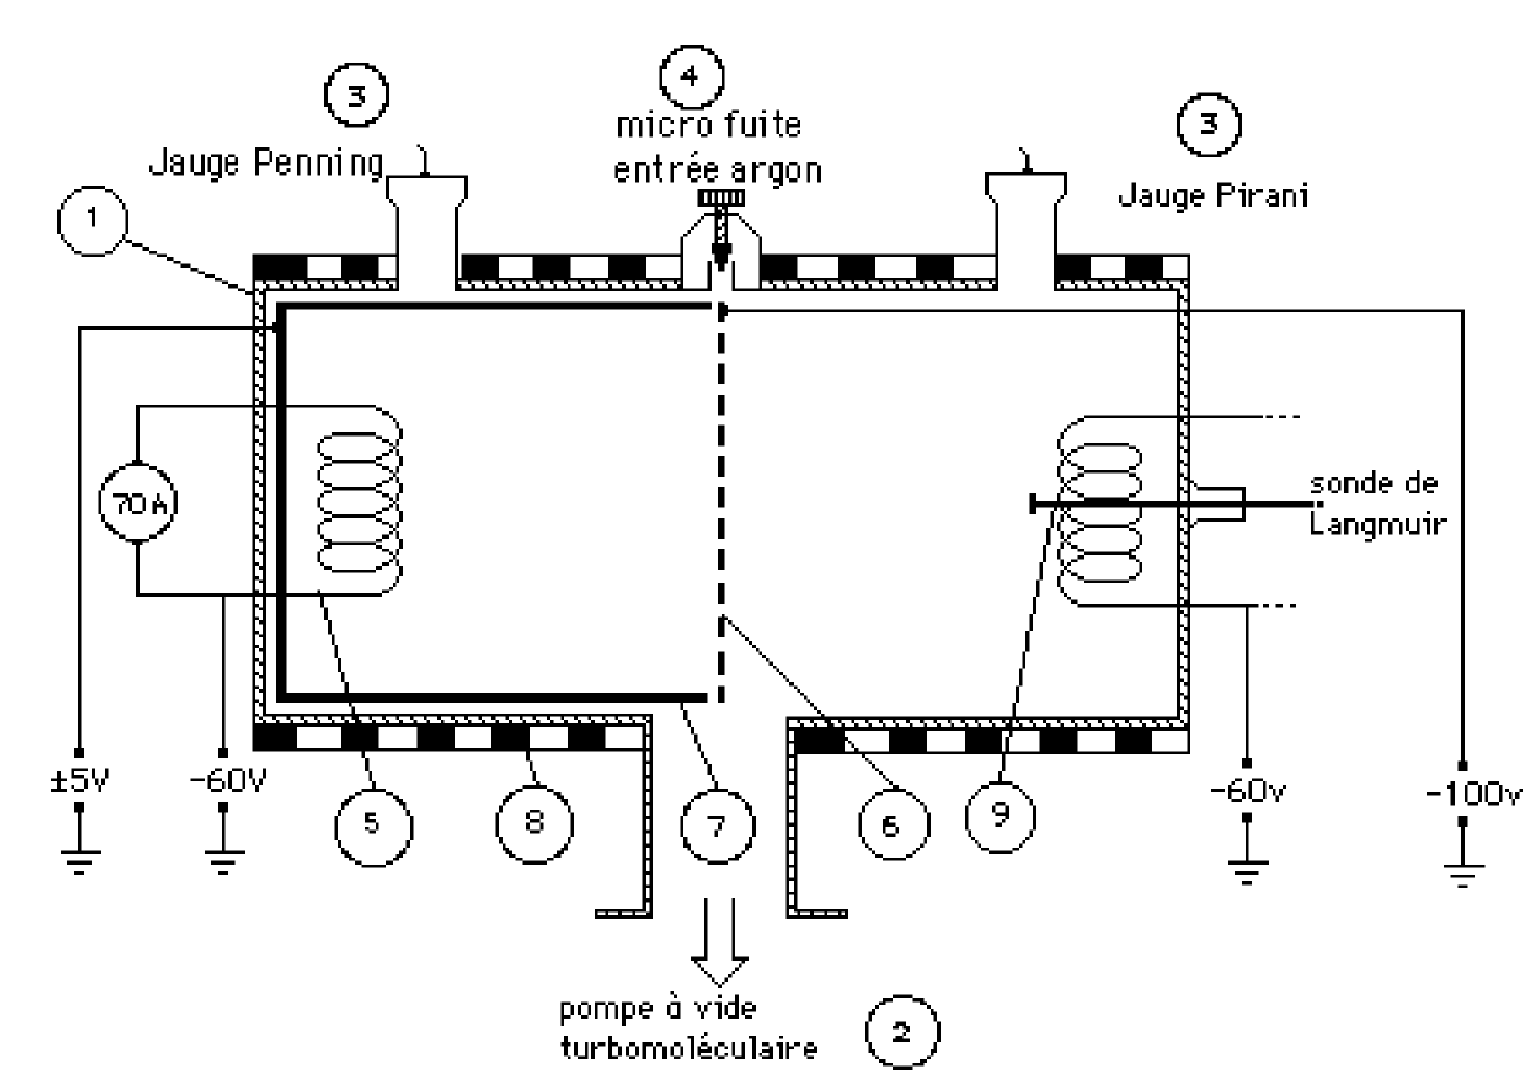
\includegraphics[width=12cm]{figures/experimental-setup.png}
    \caption{The experimental setup}
    \label{fig:experimental_setup}
\end{figure}

% The plasma is produced by electron impact ionization
% of argon atoms by electrons that are thermionically emitted and accelerated
% from a hot tungsten filament.

\cite{merlino_understanding_2007} a une explication magnifique de à quoi est-ce que ça sert les aimants.
Aussi il explique bien la courbe I-V, si on a besoin de citer quelque chose on peut balancer ça.